\documentclass[a4paper,12pt,english]{article}

\usepackage{hyperref}
\usepackage{graphicx}

\title{Renting prices and venues data analysis in Zurich, Switzerland}
\author{Nicolas, Vinard}

\begin{document}
\maketitle

\section{Introduction}
Zurich is the biggest city in Switzerland and along Hong Kong and Paris it ranks at the top of the most expensive cities in the world to live in according to the Economist Intelligence Unit's Worldwide Cost of Living report. Therefore, it is no surprise that the prices for renting apartments are very high as well. Since many jobs are in the city and it offers many cultural activities people want to live and work here. Additionally, Zurich is located at a lake which becomes a very popular spot for swimming in the summertime along with the many locations to refresh in the clear river water. \par
New residents moving to the city typically look for affordable rent and a nice neighborhood with bars and restaurants, shops, a quite residential area, good public transport connections and so on. Similarly businesses need to consider both the rent and the location. \par
We can create a map showing the rental prices in each neighborhood and cluster each neighborhood by venue type. This allows an overview of similar neighborhoods that might have a big difference in the rental costs. Additionally by viewing the results on a map other factors that are not included in the clustering can be taken into account such as the closeness of the neighborhoods to the lake, river or forests.

\section{Data}
All the data used in this project can be found online or pulled with the Fousquare API. A list of all neighborhoods, districts and their geometry can be obtained from a website managed by the city of Zurich. On that site we can also obtain a json file with the spatial information of each neighborhood that can be used to create choropleth maps of the districts, the clustering results and the rental costs. The rental costs were scraped from a realtor website RealAdvisor. The geopy library is used to retrieve the coordinates of the neighborhoods and the Foursquare API is used to get venues for each neighborhood.

\begin{enumerate}
    \item Website from the city of Zurich with information for each neighborhood such as district: \url{https://data.stadt-zuerich.ch/datase}
    \item Spatial information of each neighborhood (geo-json file): \url{https://data.stadt-zuerich.ch/dataset/geo_statistische_quartiere/resource/3c384ced-12ac-4578-b3da-bc86feb690d4}
    \item Website form which to scrape the rental prices per m2 \url{https://realadvisor.ch/en/property-prices/city-zurich}
    \begin{enumerate}
        \item BeautifulSoup used to scrape the rental prices
    \end{enumerate}
    \item Foursquare API to retrieve venues given latitude, longitude of the neighborhoods and a fixed search radius (set to 500 m here)
    \begin{enumerate}
        \item geopy used to retrieve the longitude latitude values
    \end{enumerate}
\end{enumerate}

\section{Methods}
I downloaded and saved the data from the \textit{stadt-zurich} website to my GitHub repository. With the Python library geopy I retrieved the coordinates of each neighbourhood and appended it to the neighbourhood dataframe. Next, I retrieved venues for each neighborhood using the FourSquare API. Venues within a radius of 500 meters from the coordinate of each nieghborhood are retrieved. Then I used the $k$-means algorithm to cluster the neighborhoods by venues. $k$-means is a popular unsupervised algorithm used for clustering. The optimal number of clusters, $k$ can be assessed using the so-called elbow method. For the elbow method we simply have to the algorithm multiple times for increasing $k$s and plot the value of the distortion per clusters, Fig. \ref{fig:elbow}. Finally all that is left to do is to scrape the rental costs from the realtors website and create a chropleth map of the rental costs and clusters.

\begin{figure}[h]
\centering
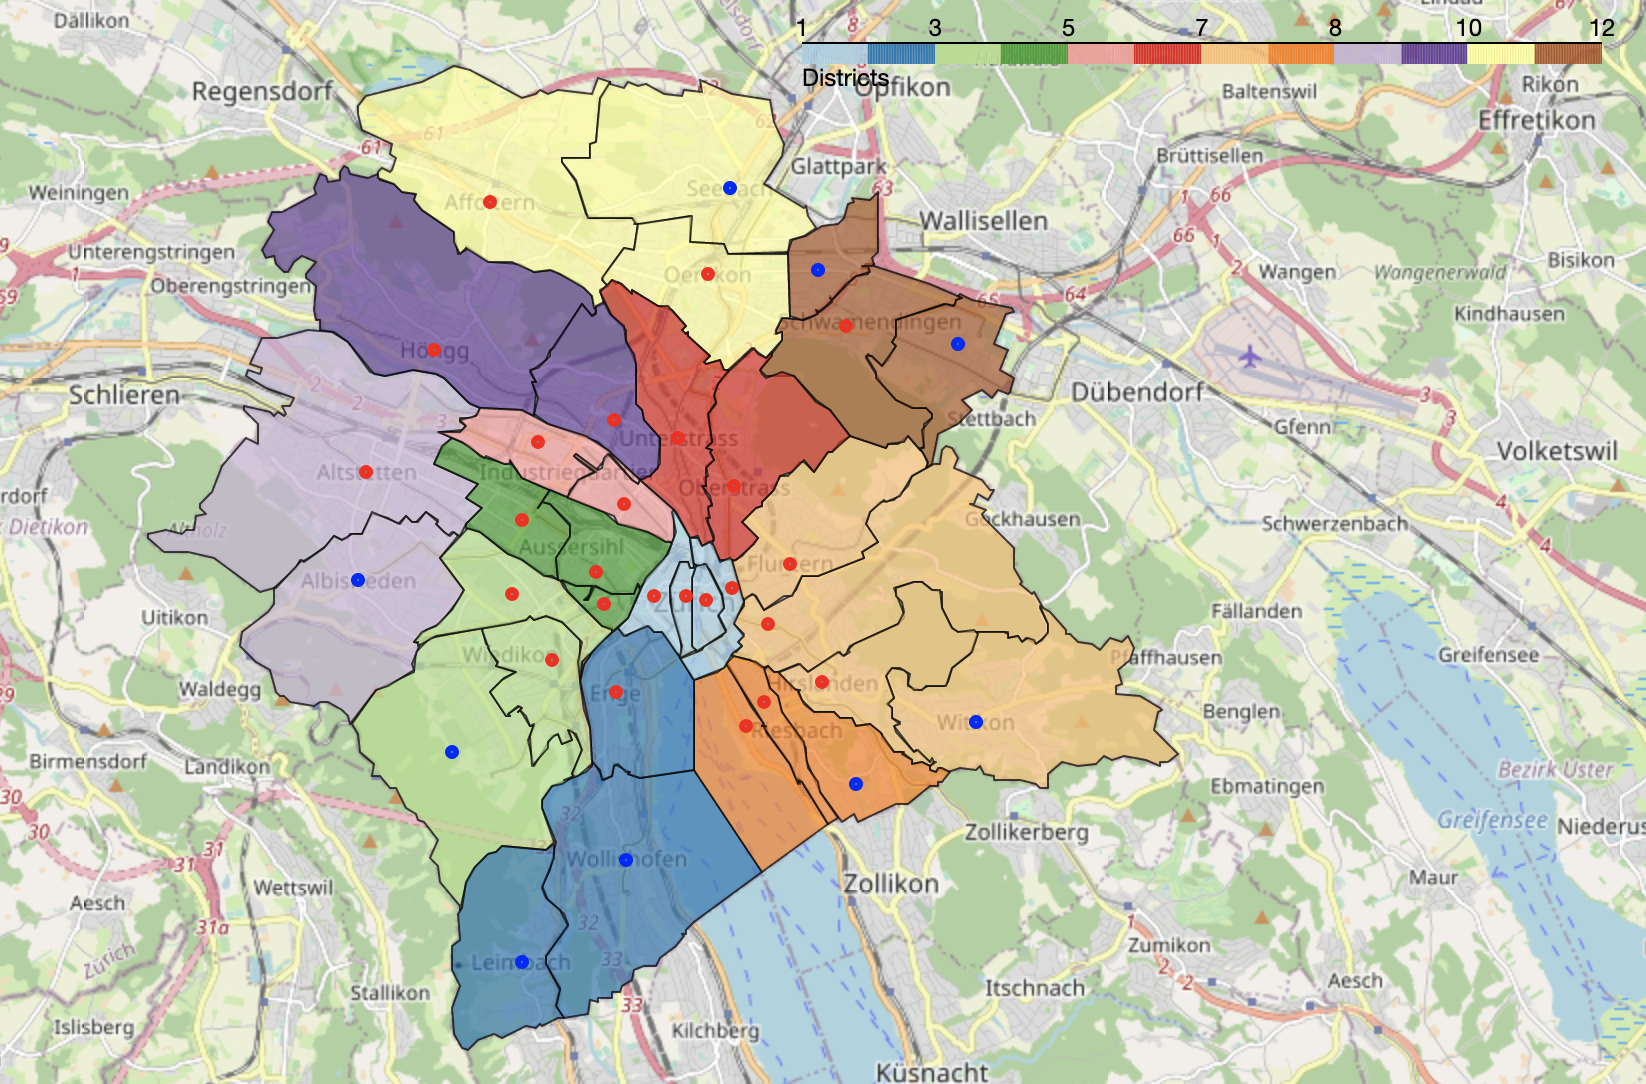
\includegraphics[width=1\linewidth]{map1}
\caption{Map showing clustered neighborhoods with red markers to denote neighborhoods with more than 10 venues and blue markers if they have less than 10 venues.}
\end{figure}\label{fig:map1}



\section{Results}
After retrieving the venues for each neighborhood we can map how many venues were retrieved per neighborhood, Fig. \ref{fig:n_venues}. We can see that the number of venues per neighborhood varies a lot (between 4 venues to 100).
\begin{figure}
\centering
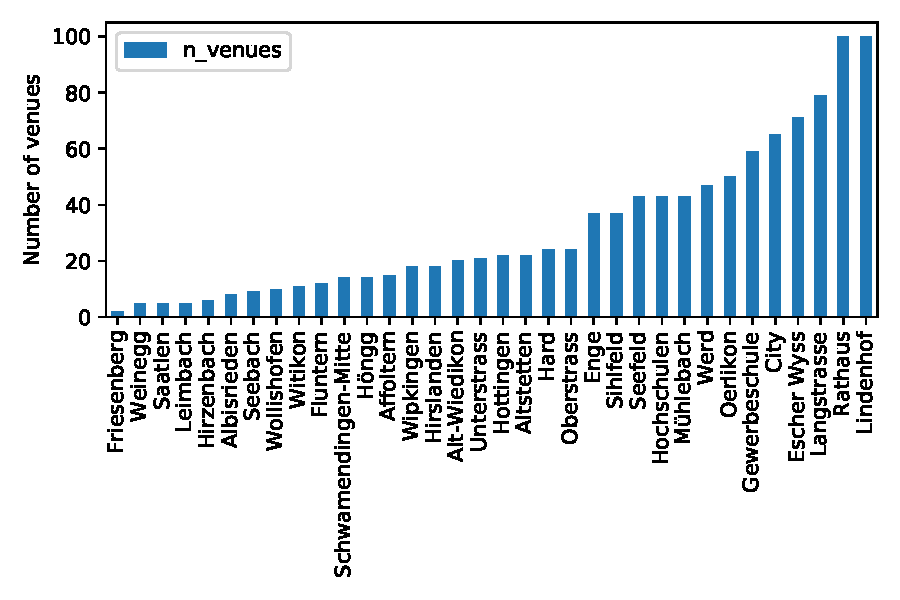
\includegraphics[width=8cm]{n_venues.pdf}
\caption{Bar chart with the number of venues retrieved per neighborhood.}
\end{figure}\label{fig:n_venues}

After retrieving the venues I used the elbow method to determine a good number of clusters, Fig. \ref{fig:elbow}. From the figure I gather that between 3 to 6 clusters are enough. I chose 6 clusters for the remainder of the analysis.
\begin{figure}
\centering
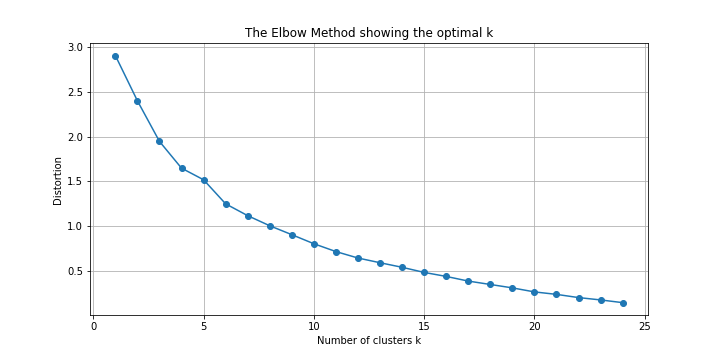
\includegraphics[width=1\linewidth]{elbow}
\caption{Elbow method applied to chose optimal k}
\end{figure}\label{fig:elbow}

The clustering result with the 6 clusters is visualized as a choropleth map in Figure \ref{fig:map2}. We see one cluster located towards the center (cluster 1) and another cluster around the outskirts (cluster 6). The remaining clusters are each composed of a single neighborhood.

\begin{figure}[h]
\centering
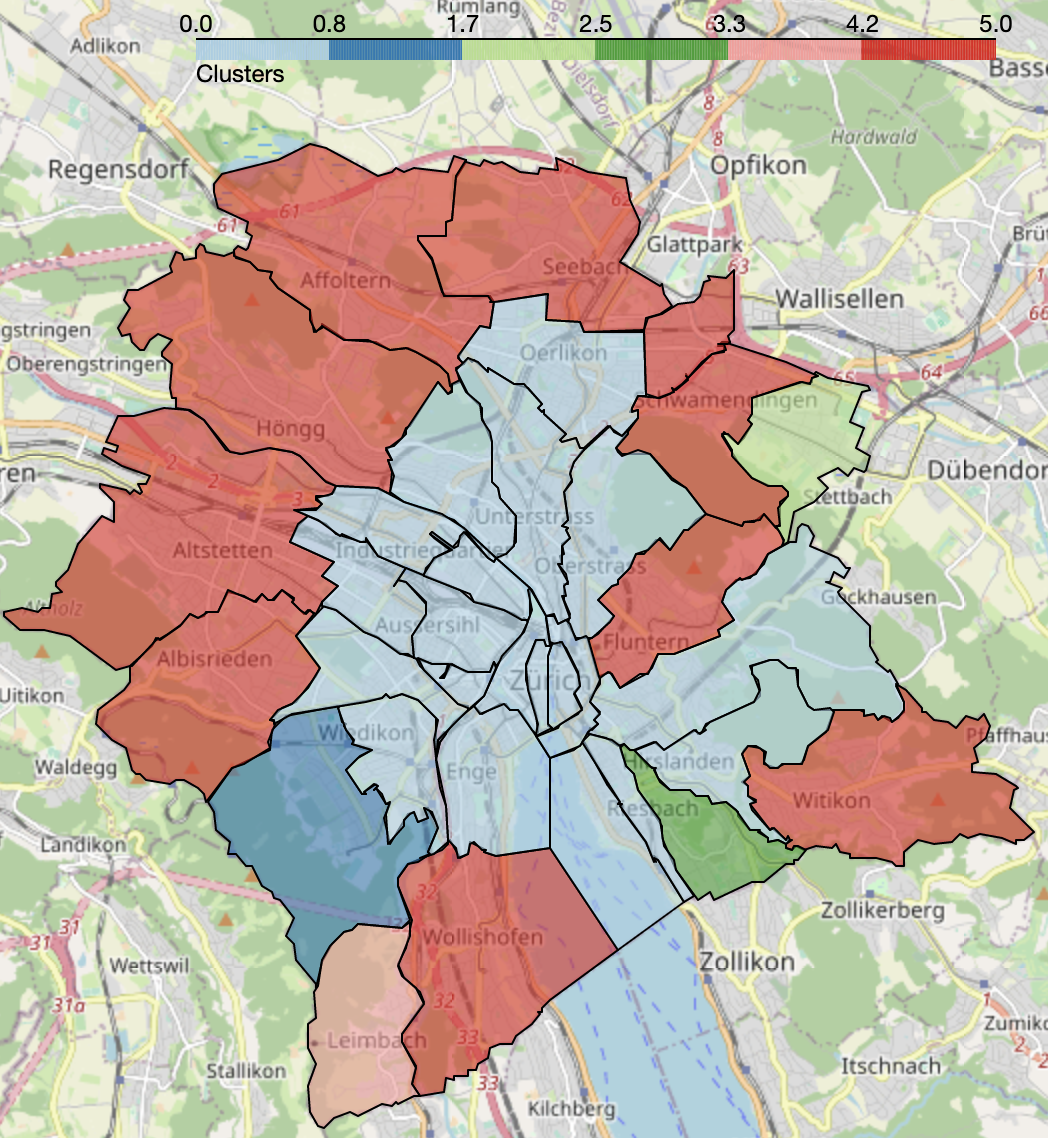
\includegraphics[width=1\linewidth]{map2}
\caption{Clustered neighborhoods}
\end{figure}\label{fig:map2}

Finally, after scraping the rental costs, a choropleth map together with the rental prices and clusters is created, Figure \ref{fig:map3}. We see that neighborhoods in the outskirts are cheapest and in the city center they are highest. The clusters also follow this trend with the first cluster being located in the city center (cyan markers) and the sixth cluster on the outskirts (red markers).


\begin{figure}[h]
\centering
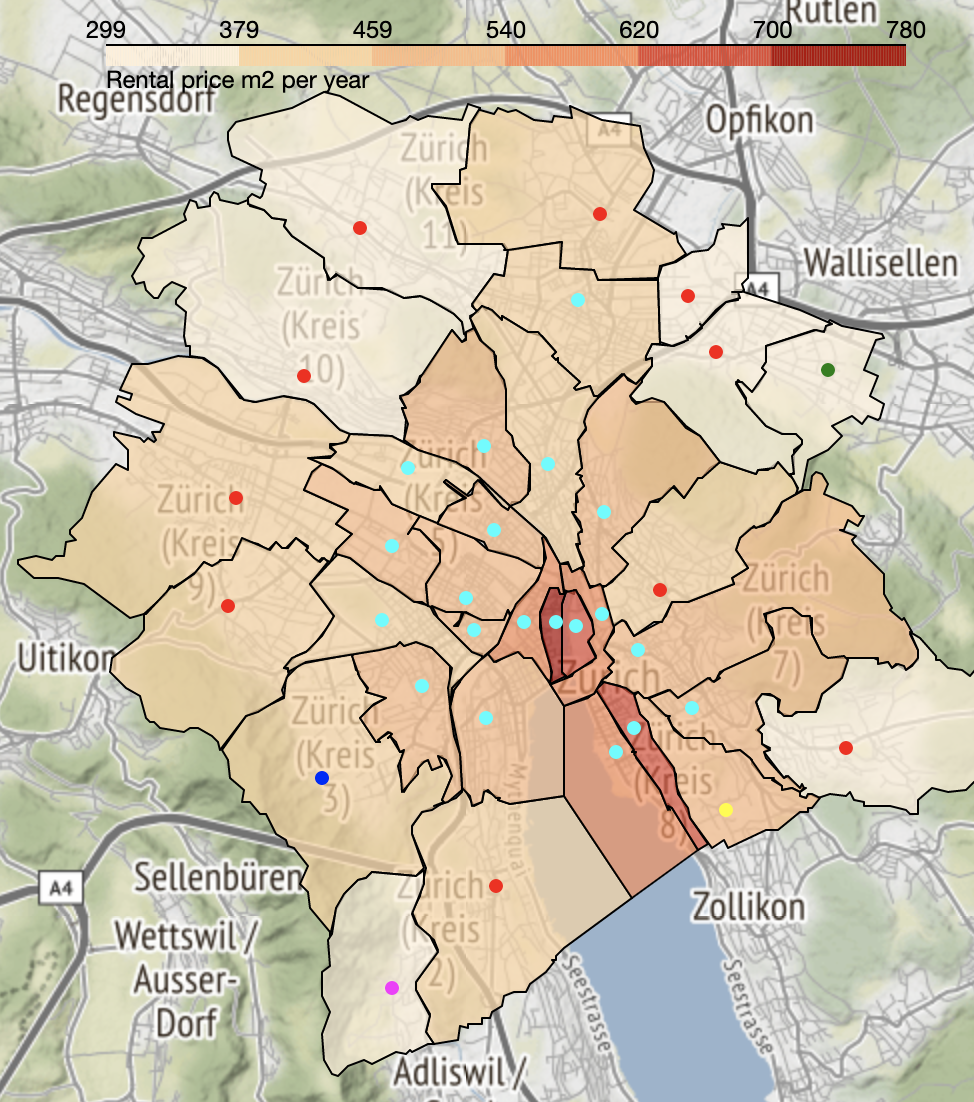
\includegraphics[width=1\linewidth]{map3}
\caption{Rental prices and clustering results: Whole neighborhoods colored by price and clusters specified by color of the marker}
\end{figure}\label{fig:map3}


\section{Discussion}
As described above I retrieved venues within a radius of 500 meters from the location of the neighborhood (latitude, longitude as returned by geopy). This is an easy way to retrieve venues for each neighborhood however, there are a couple of issues that should be kept in mind. Since all neighborhoods have different shapes and sizes, see fig. \ref{fig:map1}, venues from a large neighborhood will not be included in the search and a small neighborhood might contain venues that are actually located within its neighbouring neighborhoods. Not to forget that the maximum number of retrieved venues with a free account on Foursquare is limited to 100 per search. For some neighborhoods less than 10 venues were retrieved. I visualize these neighborhoods with a blue marker in Fig. \ref{fig:map1}. We can see that most of those neighborhoods are located within the outskirts of the city. To get most venues present in each neighbourhood I would suggest to create a grid of lonitude and latitude pairs all over the city of choice. Next, I'd retrieve the venues within a fixed radius for each geolocation and save it in a dataframe. Then I'd remove all duplicate venues. Finally, the venues can be queried given their address and added to the correct neighborhood. Certainly better ways of getting all venues per neighborhood exist but it is my first time working with the Foursquares API and this approach is currently the easiest one that I could think of. Even though some neighborhoods have a small number of venues I did not exclude them from the analysis in order to have a result for each neighborhood.\par
We can clearly see from the map in Fig. \ref{fig:map3} that the expensive neighborhoods are concentrated in the center of the city. The cheapest neighborhoods are on the outskirts of the city. Neighborhoods in cluster 1 however, show a high variation the the rental cost in the range of 379 to 798 squared meters per year. This cluster is concentrated along the city center and is characterized by a high number of bars, restaurants, hotels and coffees as expected. The cluster concentrated along the outskirts, cluster 6, is characterized by supermarkets and public transportation (buses and trams), which also makes sense. The neighborhoods are also cheaper. Finally, cluster 2, 3, 4 and 5 are each only composed of a single neighborhood. From these neighborhoods only a small number of venues were retrieved. More data (venues) should be retrieved to get better clustering results. Some of those neighborhoods have few and rare venues such as stables and tennis courts and others have only bus stations and no trams and vice versa. By generalizing venues, for instance bus and tram stations into a single category, perhaps would already lead to better clustering for these neighborhoods. Neighborhoods in cluster 2, 3 and 5 have the lowest rental costs and they are far from the city center. Cluster 4 (yellow dot in Figure \ref{fig:map3}) however, has a higher rental cost. This neighborhood has a great location by being very close to the lake and being on the east side. We can also see that the marker, which is also the geolocation, is located close to the border of this neighborhood. But we can see that a part of the neighborhood lies very close to the center where more venues are located. By placing the geolocation closer to the center of the neighborhood this hood might have been clustered with cluster 1.  \par
In this project no time was spent in pre-processing the data from the Foursquare API. Better results might be obtained if first, more venues were retrieved for some neighborhoods and second by grouping similar venues into one category. Additionally, I could have included more data such as population density, crime rates, air quality and so forth.

\section{Conclusions}
Using tools learned throughout the IBM data science specialization such as web scraping, visualization techniques and machine learning methods, allow us to analyse and visualize data with ease. The hard work lies in retrieving data, data pre-processing, using the right data analysis tools and retrieving the best insights from the results. \par
In this work I clustered neighborhoods by venues and mapped the rental prices of each neighborhood on top. The results show a correlation between the clusters and the rental costs in these neighborhoods: Neighborhoods with a small number of venues or mostly public transportation and grocery stores (typically on the outskirts of the city) tend to have low rental costs, whereas the neighborhoods with popular venues such as bars, restaurants and hotels have higher rental prices. However, the rental costs also varies greatly in these clusters. Therefore, the results can help businesses and individuals in a first step to find good neighborhoods that satisfy their needs.

\end{document}
